% Some commands used in this file
\newcommand{\package}{\emph}

\chapter{Introduction}
Quantum computing is an exciting and rapidly evolving field of modern science. One of the most promising implementations of a quantum computer is based on the ability to control and measure systems of trapped ions. Those ions are typically confined in Paul (RF) \cite{Paul1990} traps by applying static and oscillating RF signals to the trap electrodes, which on average generates a confining electric potential.
\section{Why do we need resonators?}
\label{sec:why_resonators}
One could potentially couple a radio frequency source directly to an ions' trap. However this creates the following challenges:
\begin{itemize}
	\item noise from a source may contribute to heating of trapped ions \cite{Turchette2000}
	\item in order to maintain efficient cryostat cooling amount of generated heat within it should be minimized. In order to stabilize ions in the ion trap 	confining RF signal must have a reasonably high voltage amplitude. An RF resonator close to the signal consumption area allows to reduce the length of an actively heated (with accordance to the Joule–Lenz law \cite{Prokhorov1972}) high voltage wire.
	\item impedance mismatch between source and trap leads to an additional dissipation of RF power
\end{itemize}
These issues can be avoided by placing an amplifier close to the Paul trap, which would filter the incoming signal and output it with a voltage suitable for operating the trap. There are two available options: active and passive amplifiers. Core difference between them is that active amplifiers require an additional power source to function while passive amplifiers can be used solely with a source signal itself. 

Active amplifiers perform better in terms of a voltage gain at room temperatures. However aim of this project is to create a resonator used within a cryogenic environment. Properties of transistors powering active amplifiers depend heavily on a combination of densities of free electrons and holes. Lowering the temperature tends to reduce \cite{Dirac1926} these densities significantly, turning semiconductors at room temperatures into practically dielectrics. 

It leaves us with passive amplifiers (resonators).
\section{Context of this project}
\label{sec:context}
This semester project aims to be a part of an attempt to create a scalable quantum computing architecture by Chiara Decaroli. It provides the following benefits compared to existing solutions:
\begin{itemize}
	\item using subtractive laser writing to manufacture wafers eliminates misalignment effects by allowing a ``self assembly'' of different wafers
	\item double junction ion trap designed for parallel operations, Decoherence Free Subspace (DFS) ion transport across the junctions, and manipulation of long chains of ions
	\item potential integrated laser delivery through optical lensed fibers eliminates the need for bulky optics and custom objectives which limit scalability
\end{itemize}

\begin{figure}[h]
	\centering
	\includegraphics[width=.99\textwidth]{images/trap}
	\caption{Ion trap overview (should be improved, just filling space now)}
\end{figure}

\section{Kinds of resonators}
\label{sec:kinds_resonators}
The required frequency of 40 MHz limits our selection to the following types of resonators: helical \cite{Gulde2017, Johnson2016, VanRynbach2016, Kassa2016, Kassa2017} or, for higher frequencies, coaxial \cite{Karin2012}, RLC \cite{Gandolfi2010, Kumph2015, Greene2016}, and crystal oscillators. Multiple available solutions require us to do an analysis for a reasoned choice.
\subsection{Helical}
\begin{figure}[h]
	\centering
	\includegraphics[width=.6\textwidth]{images/helical}
	\caption{Schematic diagram of a helical resonator indicating shield diameter $D$, shield height $h$, coil diameter $d$, coil height $b$, winding pitch $\tau$, and coil wire diameter $d_0$. \cite{Deng2014}}
	\label{fig:helical_example}
\end{figure}

Helical resonators are commonly selected to be coupled with ion traps due to their high quality factors and ability to operate on high frequencies. It is a perfect option for ion traps operated at room temperatures, since in absence of space constraints they are able to provide $Q$ values of a couple thousands. However in order to achieve those $Q$, the fabrication process needs to be quite precise to avoid reflections of traveling waves which negatively influence the overall gain.
\subsection{RLC}
\begin{figure}[h]
	\centering
	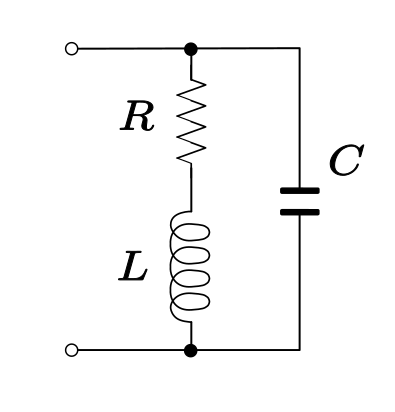
\includegraphics[width=.5\textwidth]{images/RLC}
	\caption{Example of a parallel RLC circuit}
\end{figure}

RLC amplifiers are a convenient choice for space-bounded environments, such as cryostats. Typical implementation pumps energy between two reactive components --- inductor and capacitor. Assembly of RLC circuit is easier than of helical resonator since the physical placement of lumped parts does not influence the resulting quality factor. But it also means that the quality of these components is a major factor for successful creation. Given that units' data sheets rarely provide values for cryogenic setup it takes a lot of trial and error to find the right ones \cite{Gandolfi2010}.
\subsection{Crystal}
Unlike helical and RLC resonators, the crystal oscillators do not store energy just in the electric field. This type or resonator utilizes piezoelectric effect to transform applied harmonic voltage into surface mechanical modes and vice versa.

Narrow excitation spectrum is provided by physical dimensions imposing hard constraints on vibrational oscillations and could have made such device an ideal filtering solution for ions traps. Unfortunately, there are some major downsides that seriously limit its applicability:
\begin{itemize}
	\item after fabrication resonant frequency can not be widely tuned
	\item limited stability of the crystal does not allow high voltages
\end{itemize}
\subsection{Choosing the right one}
In our setup, the combination of high voltage and frequency values with our constraints on available space makes helical resonator the optimal option. However, difficulties of assembly do not make it a perfect solution in terms of scalability --- for a production-grade setup RLC amplifier might be preferred.

\begin{figure}[h]
	\includegraphics[width=\textwidth]{images/4K_chamber}
	\caption{3D model of a 4K cryostat chamber}
	\label{fig:4K_chamber}
\end{figure}